\pagestyle{empty}

\chapter*{外\quad 文\quad 译\quad 文}

\begin{center}
{\heiti\zihao{3}Distributed Semantic Web Data Management in HBase and MySQL Cluster \\
\textsl{By Craig Franke, Samuel Morin, Artem Chebotko, John Abraham, and Pearl Brazier}

\heiti 在HBase和MySQL集群中的分布式语义WEB的数据管理
}
\end{center}

\zihao{-4}

\section*{摘要}
在互联网上的各种各样的计算型资源和数据资源正通过机器解释的语义描述方式得到增强,以便于更好的搜索、发现和集成。这个由相互关联的元数据构成的语义Web,它的容量能潜在地增加着整个互联网的规模。语义Web数据的高效管理,通过W3C的资源描述框架进行表述,对于支持新型的数据密集型语义的应用来说是非常关键的。在本次工作中,我们研究并比较了两种基于新兴的云计算技术和传统的关系型数据集群技术的分布式RDF数据管理方法。特别的,我们为HBase和MySQL集群设计了分布式RDF数据存储和查询方案,并且在the Third Provenance Challenge和Lehigh大学的机器集群上通过使用基准数据集和查询对这些方法进行了实证比较。我们的研究结果揭示了有趣的查询评估模式,这表明了我们的算法是拥有前途的,而且暗示了对于可扩展的语义Web数据管理来说云计算有很大的潜力。


\section*{综述}
  万维网联盟(W3C)推荐并标准化了一系列的规则则、语言、框架和连接各种各样的元数据到下一代互联网的最佳实践,那就是语义Web。W3C的元数据获取语言包括资源描述框架(RDF),RDFa(属性),RDFs(模式),Web本体语言(OWL)。政府、学术界和产业界积极的拥抱这些技术来捕获和共享语义Web的元数据。举几个例子,oeGOV正在为电子市场制定和发布OWL本体,美国人口普查数据正以RDF的形式发布,生物信息学家以RDF的方式维持通用蛋白质资源,地球科学家出版全球范围的地里的RDF数据库GeoNames,美国最大的电子产品零售商百思买以RDF的方式发布它所有的产品目录,美国最大的社交网络提供商Facebook使用RDFa在它的网页中嵌入元数据。服务计算社区通过使用了例如OWL-S、WSDL-S、SWSO等词汇的语义注释,增强了现有的语义Web服务。


  RDF数据模型是一个直接的,标识的图形,他也可以被序列化为一组三元关系。本论文中的例子包括10个描述了使用LUBM词汇的三元组,如图1所示。每个三元组由一个主体,谓词和对象组成,并且定义了一个主体和对象之间的关系。图中<>和“”分别表示资源标识符和一些个数据类型。例如,前三个三元组的资源标识符C是一个学生,拥有名字Craig并且是IEEE的成员。这个示例数据集可以使用SPARQL语言来查询,它是一个RDF的标准查询语言。SPARQL使用三元模型和图形模型来匹配RDF数据。例如从包含?X< type ><UndergraduateStudent>模式的LUBM中的Q14查询返回所有本科生标志并赋给X变量。关于SPARQL特性和语义更多的细节可以在W3C的SPARQL规范中发现。

  随着语义Web的快速发展和作为元数据的主要语言的RDF的广泛应用,RDF数据有效的管理将会对于支持新型的在不同领域的语义应用来说是至关重要的。许多研究人员建议使用关系型数据库存储和查询大型的RDF数据集。这种被称作关系型RDF数据库或者关系型RDF商店的系统现在正被频繁地应用在产品中。最近,在云计算中广泛使用的分布式技术如Hadoop何Hbase等,正用来开发分布式的和可扩展的RDF数据管理。据我们所知,这项工作提供了在Hbase和MysQL集群中使用我们的设计和算法解决方案来进行存储和查询RDF数据的关键性能的比较。

  本篇论文的主要贡献有:(i)用来在HBase中存储RDF数据的新型数据库结构设计(ii)为由我们设计的模式在HBase中进行SPARQL三元组和基本图形的模式匹配提供了有效的算法(iii)高效的SPARQL和SQL之间转换的算法,它能使MySQL集群上进行的SQL查询变得平滑(iv)HBase和MySQL集群上存储和查询语义Web数据的高效和可扩展性的富有经验性的比较。我们的工作展示了在查询评估中有趣的模式,这表明了我们的算法是有希望的,并且暗示了云计算对于可扩展的语义Web的数据管理来说有很大的潜力。

  本篇论文的组织如下:在第二章介绍了相关的工作,第三章和第四章介绍了我们对于HBase和MySQL集群上进行分布式RDF数据的存储和查询的设计和算法,第五章介绍了这两种方法在the Third Provenance Challenge 和Lehigh 大学进行的基准数据集的性能测试报告。最后我们在第六章进行了总结。


\section*{相关工作}
  除了作为google的Bigtable开源实现的HBase,还有很多在Apache基金会下的项目,他们将焦点地方在分布式的计算,这些项目包括Hadoop,Cassandra,Hive,Pig和CouchDB。Hadoop实现了MapReduce软件架构和分布式文件系统。Cassandra将一个完全分布式的设计和面向列的存储融合起来,并且将MapReduce作为支持的特性之一。Hive在Hadoop之上处理数据仓库并且提供了他自己的查询语言HQL。Pig面向于使用它的高层的Pig拉丁语言来书写数据分析程序,这些程序最终被转化为MapReduce工作,以此完成分析大型的数据集。CouchDB是一个分布式的、面向文档的非关系型数据库,它支持JavaScript编写的增量性的MapReduce查询。在学术界和工业界的其他项目,包括Cheetah, Hadoop++, G-Store和HadoopDB都有类似的思路。

 
  接下来简要讨论一下关于分布式RDF数据管理的一些相关工作。参考文献3和6里呈现了评估SPARQL的基本图形模式的技术。参考文献7和8分别提出了在以MapReduce系统中分析型查询处理和RDF图形分布式推理的有效方法。参考文献9和10研究了在点对点的环境下RDF查询处理,11和12报告了分布式RDF源之间联合查询的调解技术。13介绍了在文本索引中HBase的用处。在参考文献14中虽然S声明了spider系统使用了HBase来处理RDF查询处理和扩展的HBase,但是并没有详细的报告。最后,我们之前的工作展示了在HBase中RDF数据管理的最初发现。这篇论文提出了更新更有效的HBase表结构设计,更高效的SPARQL三元组和基本图形模式匹配和算法和对于分布式关系型RDF数据库富有经验的比较。我们的实验比较结果呈现出对于一些查询的数个数量级的提高,以及可扩展性的重大改进。这篇论文和我们之前的论文是关于HBase中语义Web数据管理最先发表的研究成果。我们对于HBase和MySQL集群的RDF数据管理技术的比较也是独一无二的。 

\section*{在Hbase中的分布式RDF数据存储和查询}
  Hbase将数据存储在表中,并且数据可以表述为非常稀疏的多维的排序的映射,这和传统的关系型数据库里的关系非常不同。一个Hbase里的表存储了根据rowkey排序的数据行。每一行有一个唯一的rowkey和任意数量的列,这样在两个不同行的列就不用一模一样。一个列的完整的名称包括一个列族和一个列修饰符,这里的列族是在表建立时就指定的,列族的数量是不会变的,但是列修饰符却可以动态的增加和删除。一个给定行的一列,我们称之为表单元格,能存储一对时间戳值,时间戳在单元格里是惟一的,并且值可以重复。表中的行在Hbase集群不同的机器上可以成为分布式的,并且能进行两个基本的操作:1.表的扫描 2.根据一个给定的rowkey或者列、时间戳等等来检索表格的数据。考虑到对于大数量级来说表格扫描访问路径是非常低效的,以rowkey来检索是最有效的方法。

  
  表格稀疏的特性使得它们称为RDF数据非常富有吸引力的存储选择。RDF图表通常也是很稀松的:不同的资源用不同的属性来注释,并且一些注解可能由于推理的缘故不会显示的指出。为了支持在Hbase表中有效的检索RDF数据,应该考虑到SPARQL构造的基本查询,比如三元模式等等。数据库最起码应该支持RDF三元组的主体、谓词、对象的值的检索。


  我们建议使用两个表的数据库模式来存储RDF三元组,正如图2所示。sp表存储了三元组的主体作为rowkey,三元组的谓词作为列名字,三元组的对象作为单元格的值。op表存储三元组的对象作为rowkey,三元组的谓词作为列名字,三元组的主体作为单元格的值。表2显示了使用我们RDF三元组样例来存储这些表的二维的图形化展示。在这幅图里,s和o代表了rowkey而不是列;类型,名字,属于什么组是列修饰符,这些修饰符属于共同的列族p;{}代表了省略了时间戳的单元格值的集合。更加确切的说,行的这种表结构可以用JavaScript 对象符号来表示为:
\begin{lstlisting}
//the first row of Tsp
<C>:{
  p:{
	type: {t1: <Student> },
	name: {t2: "Carig" },
	memberof:{t3: <IEEE>}
 }
}
//the first row of Top
<Student>:{
 p: {
	type:{ t4:<C>,t5:<S>}
	}
}
\end{lstlisting}

RDF数据建议的模式要求数据本身被存储两次以便用来保证系统的健壮性。表Tsp和Top分别可以根据一致的主体或对象来有效的检索三元组信息。而基于一个谓词的值的检索,由于他需要一个表的全表扫描,因而可能不会非常有效。为了解决这个问题,我们可以创建表Tps或Tpo,将谓词放在rowkey的位置上,而将主体或对象作为列。然而,这样的解决方法只能提供轻微的改善,因为本体的谓词数量通常是比较固定的且相对很小的,这暗示了新的表只能包含大量行的一小部分,而对于任何单一行的检索仍然是代价昂贵的。

为了使Hbase能够评估SPARQL查询,我们设计了三个函数来处理三元组模式和基本图表模式。

我们的第一个函数叫做matchTP-T,是一个通用的函数,它既不依赖于我们的存储模式也不依赖于Hbase。matchTP-T将一个三元模式tp和一个三元组t作为输入,如果他们匹配则返回true,否则返回false。它的伪代码在4中呈现。

算法1中的函数matchTP-DB是用来根据我们的两个表的存储模式来匹配HBase数据库DB中的一个三元组模式tp。这个函数的输出是一个多重集合B,它包含了数据库中所有匹配的三元组。这个算法处理三个不相关的例子。首先,如果tp的主体模式不是一个变量,这个函数从Tsp表中检索出结果。如果tp.pp不是变量,只有拥有了列修饰符tp.pp的列的值从行中检索出来。否则,所有的列都将被检索。由于tp.op可能是也可能不是一个变量,matchTP-T被用在所有的三元组上以除去不匹配的组。在这个过滤之后,B中的组被返回。第二,如果tp的对象模式不是一个变量,这个函数使用相似的方法从表Top中检索出数据。最后,当tp.sp和tp.op都是变量时,其中的一个表必须扫描来检索出所有的行。如果tp.pp不是一个变量,不匹配的列将被舍弃,否则,所有列中的值都将被使用。

  我们最后一个函数matchBGP-DB在算法2中给出轮廓。它将包含了一系列三元组tp1,tp2...的SPARQL基本的图表模式bgp和HBase数据库进行比较,并且返回一个由匹配的三元组组成的图表集合B。这个算法首先使用两个准则来排序bgp中的三元组:(1)为了减少迭代的次数首先应将产出结果小的三元模式放在首位,(2)为了避免不必要的笛卡尔积应将那些有共同变量的三元组优先考虑。作为一个例子,考虑下面的查询和它的排序版本。原来查询中的顺序并不符合所需的条件:tp1在数据集里产生了大量的所有大学里的学生的结果集;tp2和tp1没有公告变量,并且在tp1和tp2之间必须计算耗费内存的笛卡儿积;被记录的查询既能节省内存又能节省网络传输时间:对于三元组tp3,它不仅仅因为有最小结果集它被放在第一位,而且笛卡尔积也被移除了。

  接下来,这个算法使用matchTP-DB算法来评估bgp里的排好序的第一个三元组。如果B中的结果为空,这个算法就不再评估它的子三元组而返回一个空结果集。否则,matchBGP-DB函数就会迭代地计算三元组或者公共变量或者没有公共变量时计算笛卡尔积。每个join连接就像关系型数据库中的连接策略。公共变量首先被B集合中绑定的替换,并使用matchTP-DB函数评估TP集合中的三元组tp'。如果tp'生成了非空的结果,B'中的三元组就将B中相应的三元组串联在一起。

\section*{在Mysql集群中分布式RDF数据存储和查询}
关系型RDF数据库使用几种数据模式产生的方法,包括schema-oblivious,schema-aware等等。这些方法标志了不同的数据库关系,比如属性,类,类的主体和客体及集群化的数据库表等等。在这项工作里,我们使用schema-oblivious方法作用到单个表T(s,p,o)上,这里的列s,p,o相应的存储了三元组的主体,谓词,对象。

  我们选择这一个模式是由于三种原因。首先,它可以支持无模式的修改本体演化。Hbase建议的模式也是非常灵活的,因为只有列的修饰符才会动态的变化而且是在行级上进行变化的。第二,关系型RDF数据库中涉及到的大部分表都可以看作是表水平分区的结果。然而,分区的工作已经被Mysql集群自动的进行了。最后,这个模式允许无损存储,并且很容易实现,特别是它大大的简化了SPARQL到SQL的转换工作,这个工作需要查询存储的RDF数据。

  为了在Mysql集群的数据库架构上执行SPARQL查询,我们提出了一个基本图表模式的SPARQL到SQL的查询转换算法。该算法是以我们以前的工作15为基础,但是它又进行了优化,以生成平坦的SQL查询。平坦的查询会移除一系列在基本图表模式上重新排序的三元组,因为关系型的查询优化器足以自动地选出一个好的连接查询执行序列。

\section*{性能研究}
这一章讨论了在HBase和Mysql集群上进行分布式存储和查询RDF数据的不同方法的经验性比较。
A.实验前提
硬件。我们的实验使用9个有着标准硬件的商业机器。每个机器有3GHz 64bit的奔腾四核处理器,2GB DDR2-533RAM,80GB 7200转串行ATA硬件驱动。机器通过网络连接到一个戴尔巨型以太网交换机,该交换机上安装了64位的Debian Linux和Oracle JDK6。
HBase和Mysql集群。使用了带有更改内核库的Hadoop0.20.2,还有HBase0.90.为了稳定性我们对默认的配置做了细微的更改,包括设置每个数据块复制两次,增加HBase最大堆大小到1.2GB。同时使用了基于快速入门指南配置上更改的Mysql集群7.1.9a,将NDB数据节点使用的内存增加。
我们的实现。我们的算法使用Java语言来实现,并且实验通过使用Bash脚本来自动地和可重复地执行Java类文件和存储的结果。
查询性能评估。Hbase和Mysql集群在PC3和LUBM数据集上的查询性能和可扩展性结果在图4上报告。PC3基准测试送三个不同复杂性的查询:Q1是最简单的查询只用了一个三元组。Q2有三个三元模式,Q3是最复杂的,包括6个模式。所有三个查询里基本的图表模式返回一个小量结果。Hbase和Mysql集群都显示出非常有效的响应时间,而前者稍微的快一点。在第六天,Hbase之前保持的持平的时间也有了轻微的上升,这意味着图有一个小的斜坡(数据集的大小增加了近10倍,而响应时间只有大约2~4倍的增加),类似的行为也在LUBM查询中观察到。

\newpage
\section*{外文译文原文}

\begin{figure}[!ht]
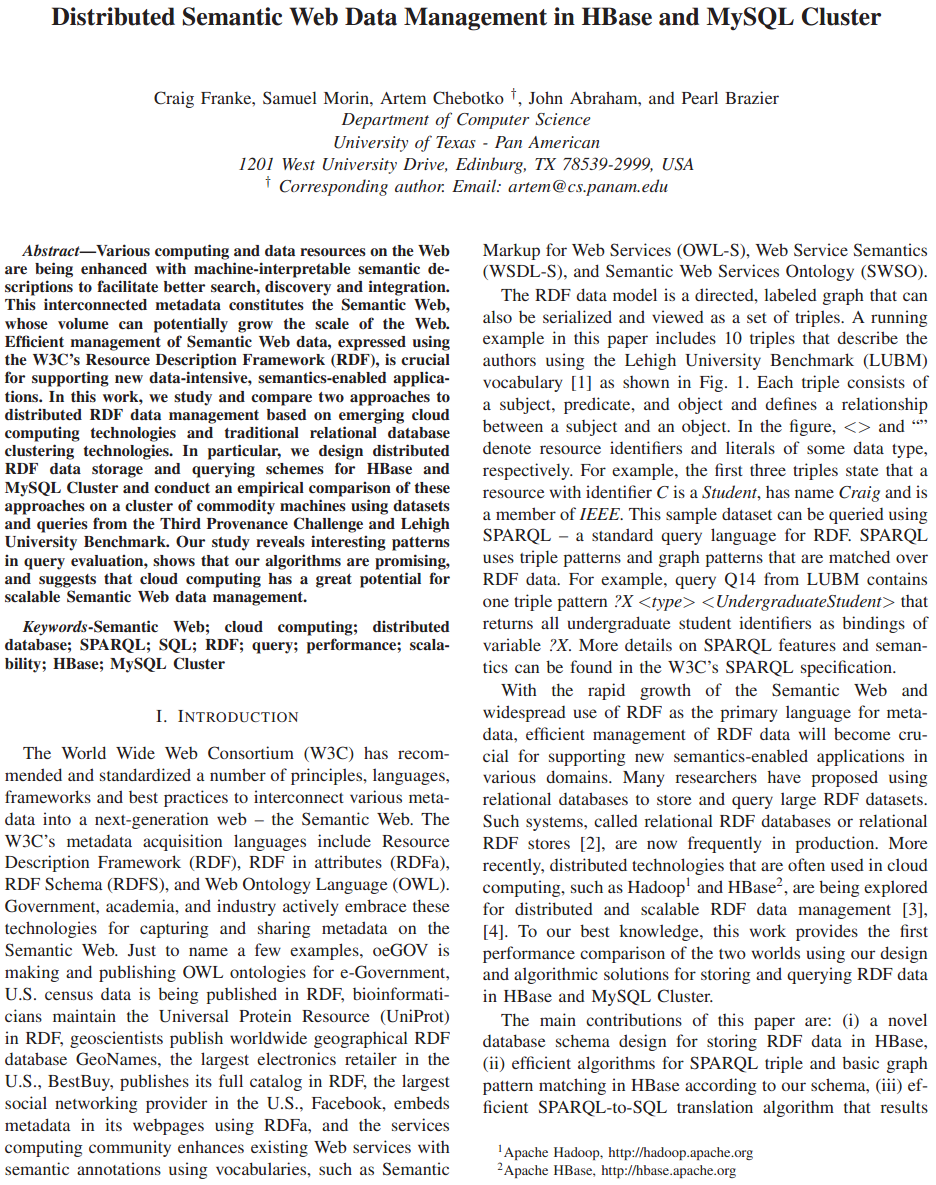
\includegraphics[scale=0.67]{photo/yingyu1.png}
\end{figure} 

\begin{figure}[!ht]
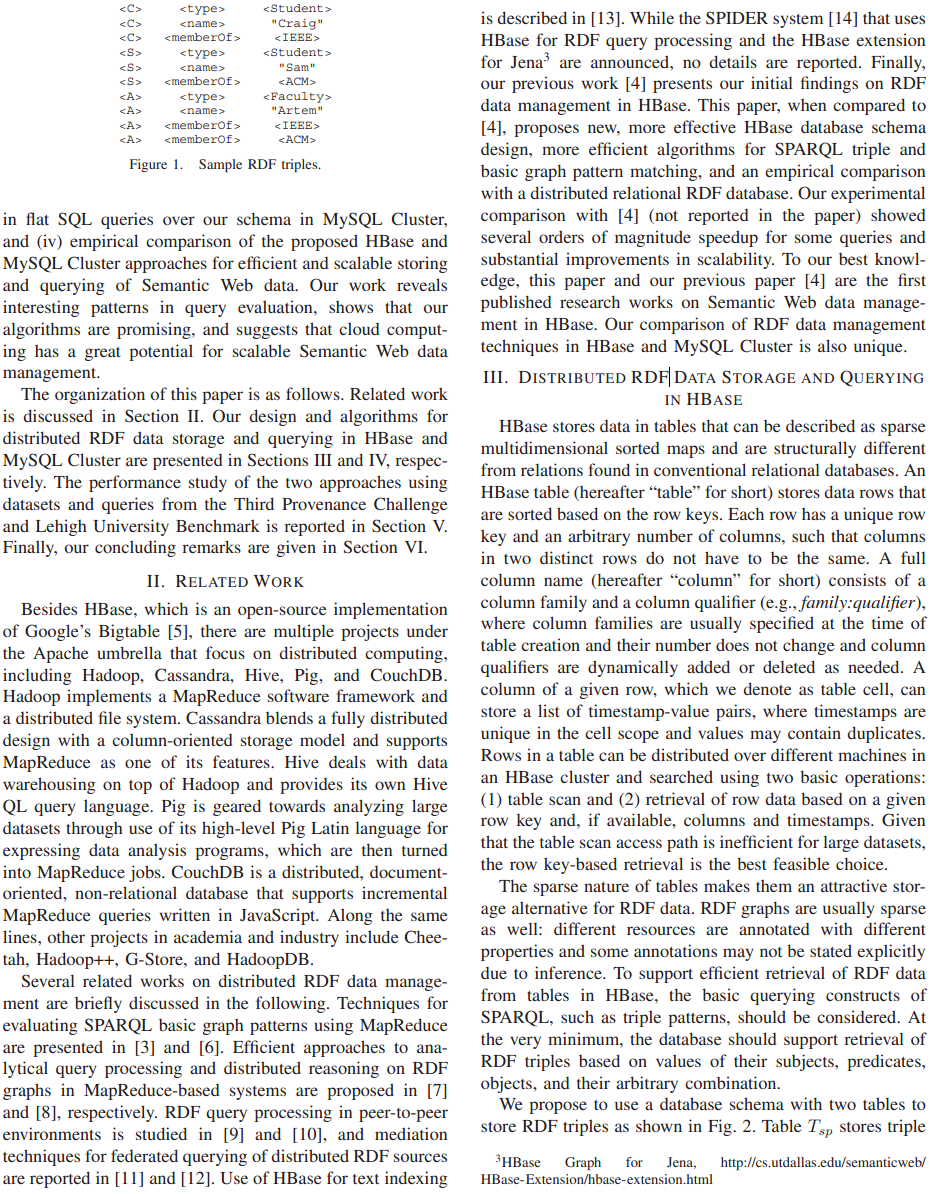
\includegraphics[scale=0.67]{photo/yingyu2.png}
\end{figure} 

\begin{figure}[!ht]
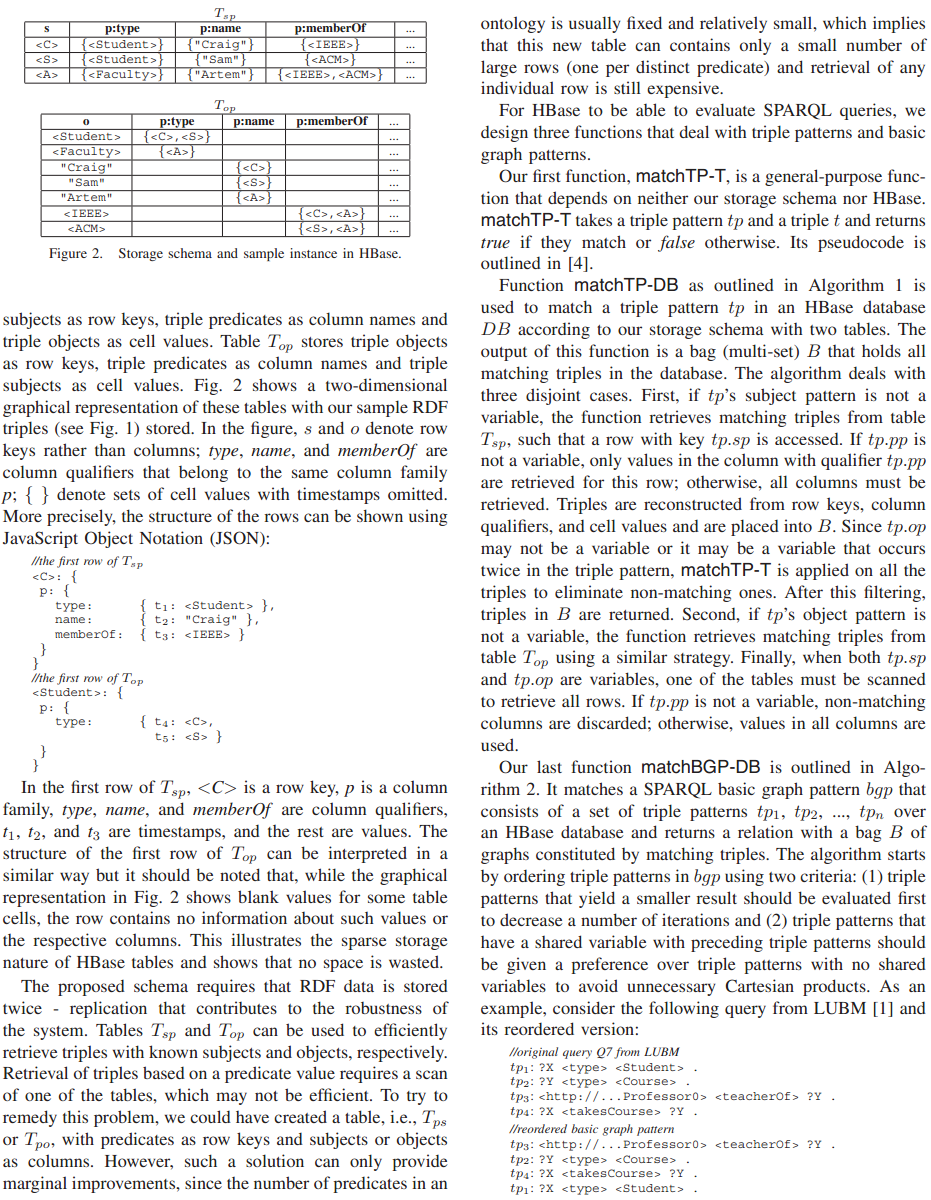
\includegraphics[scale=0.67]{photo/yingyu3.png}
\end{figure} 

\begin{figure}[!ht]
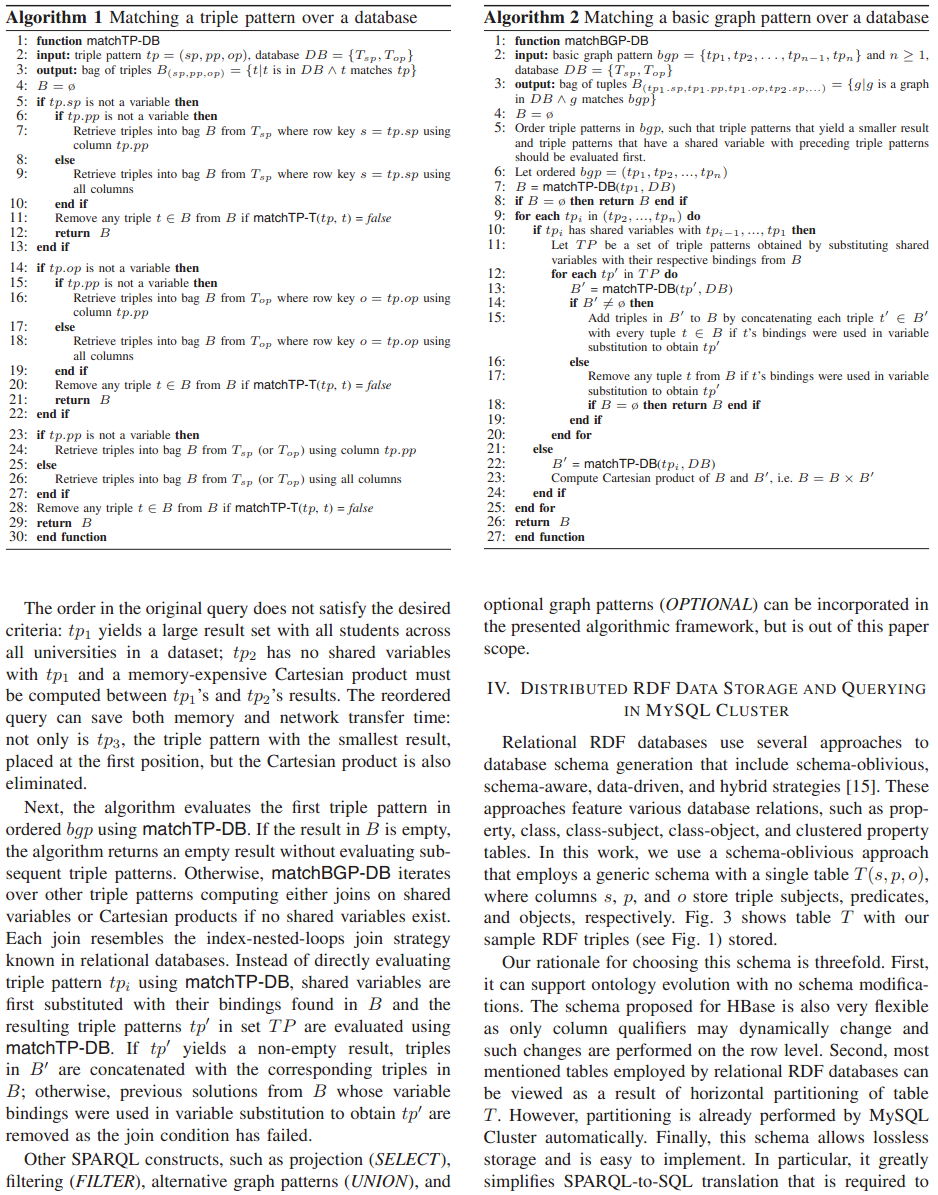
\includegraphics[scale=0.67]{photo/yingyu4.png}
\end{figure} 

\begin{figure}[!ht]
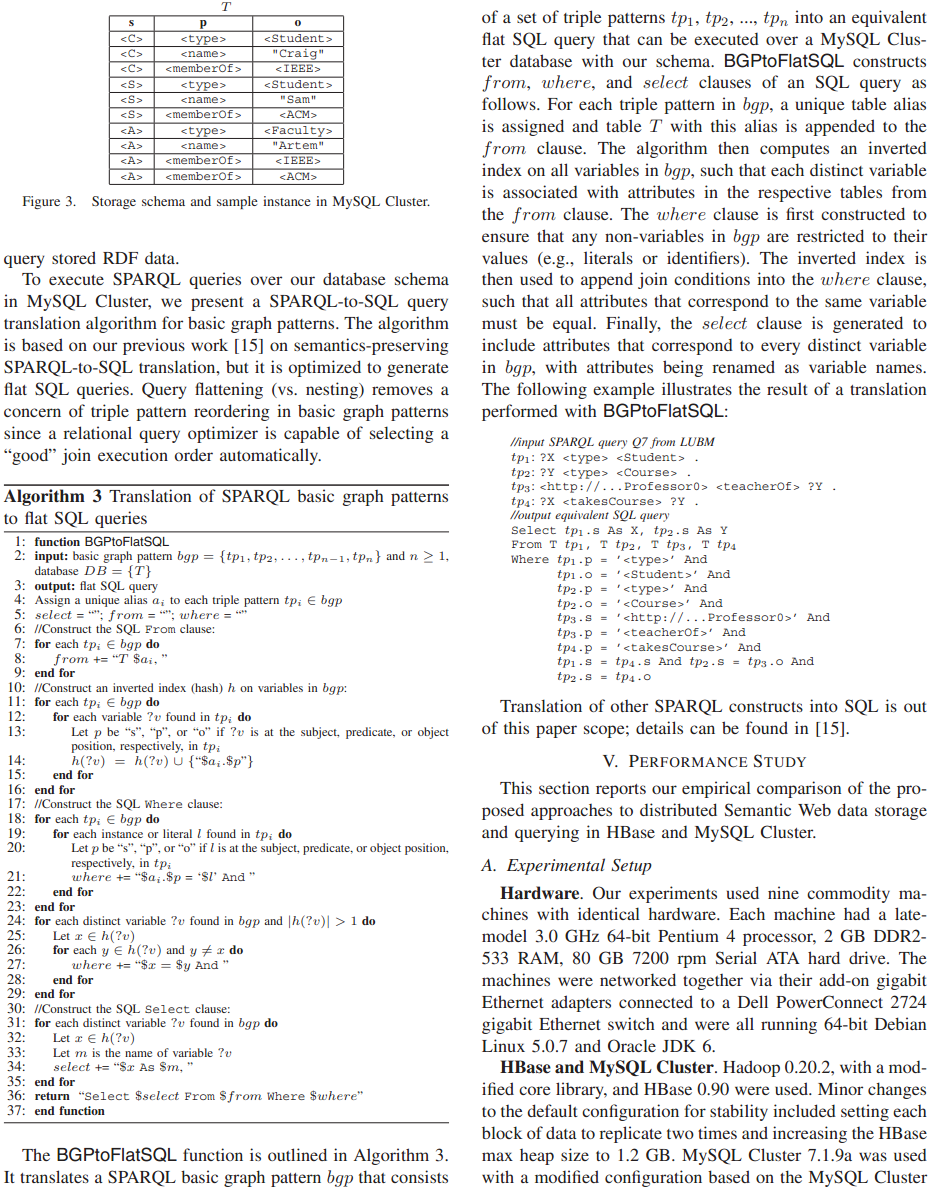
\includegraphics[scale=0.67]{photo/yingyu5.png}
\end{figure} 

\begin{figure}[!ht]
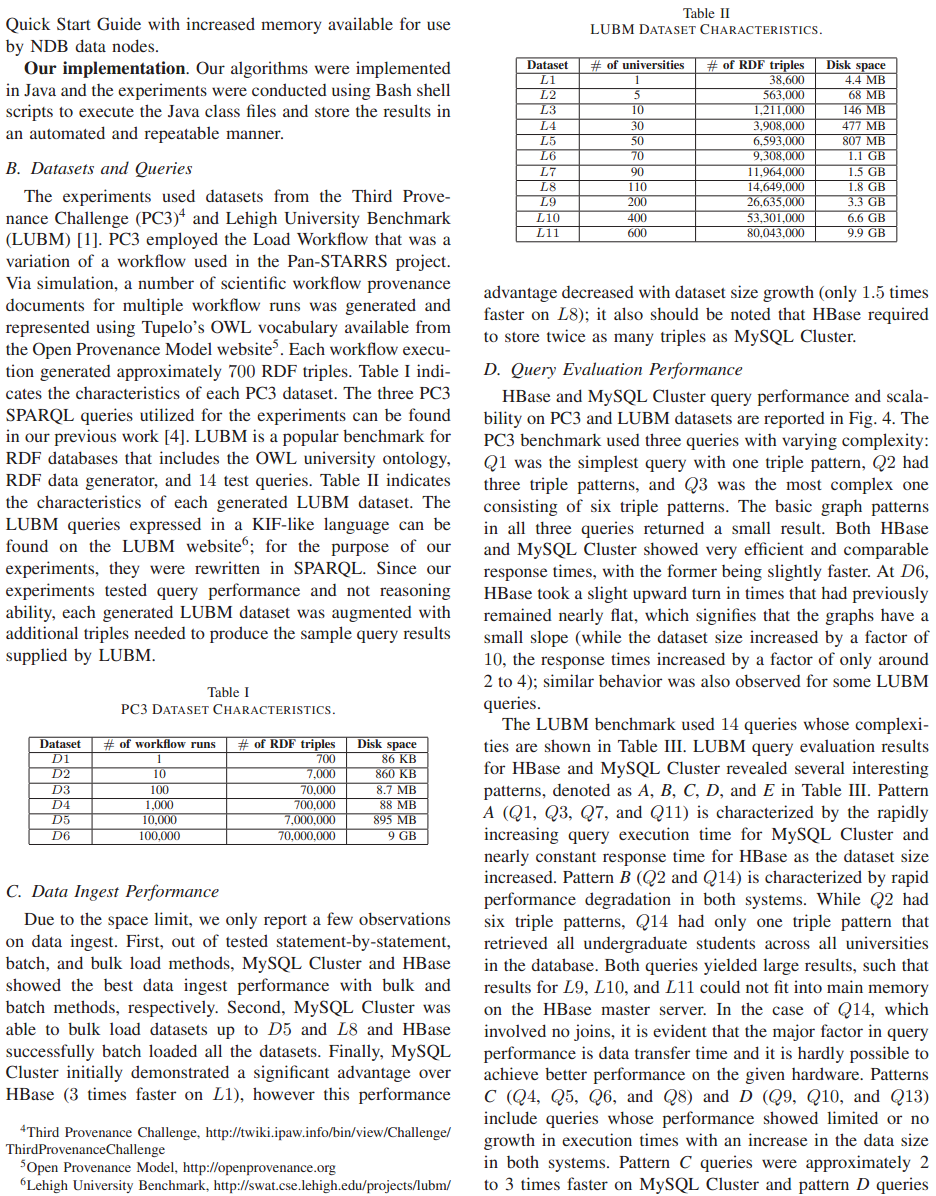
\includegraphics[scale=0.67]{photo/yingyu6.png}
\end{figure} 

\begin{figure}[!ht]
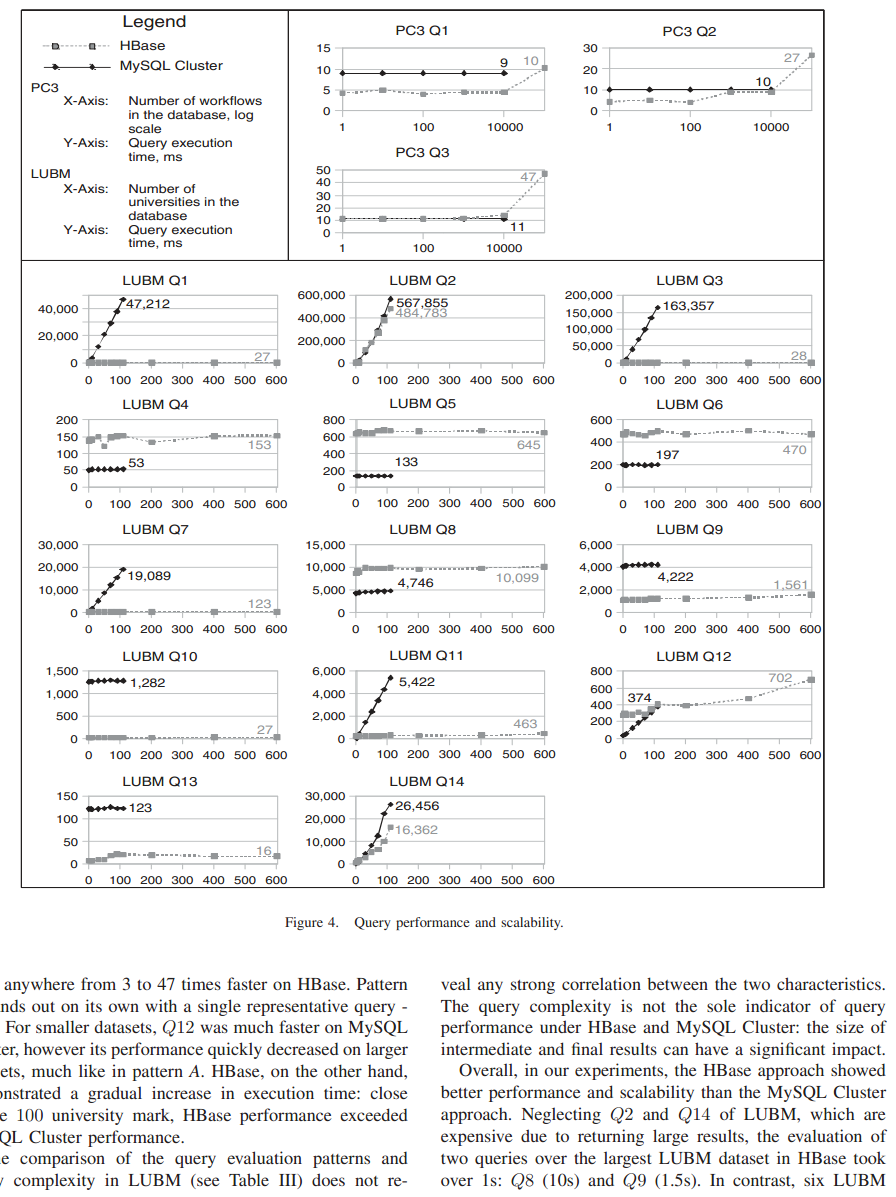
\includegraphics[scale=0.67]{photo/yingyu7.png}
\end{figure} 

\begin{figure}[!ht]
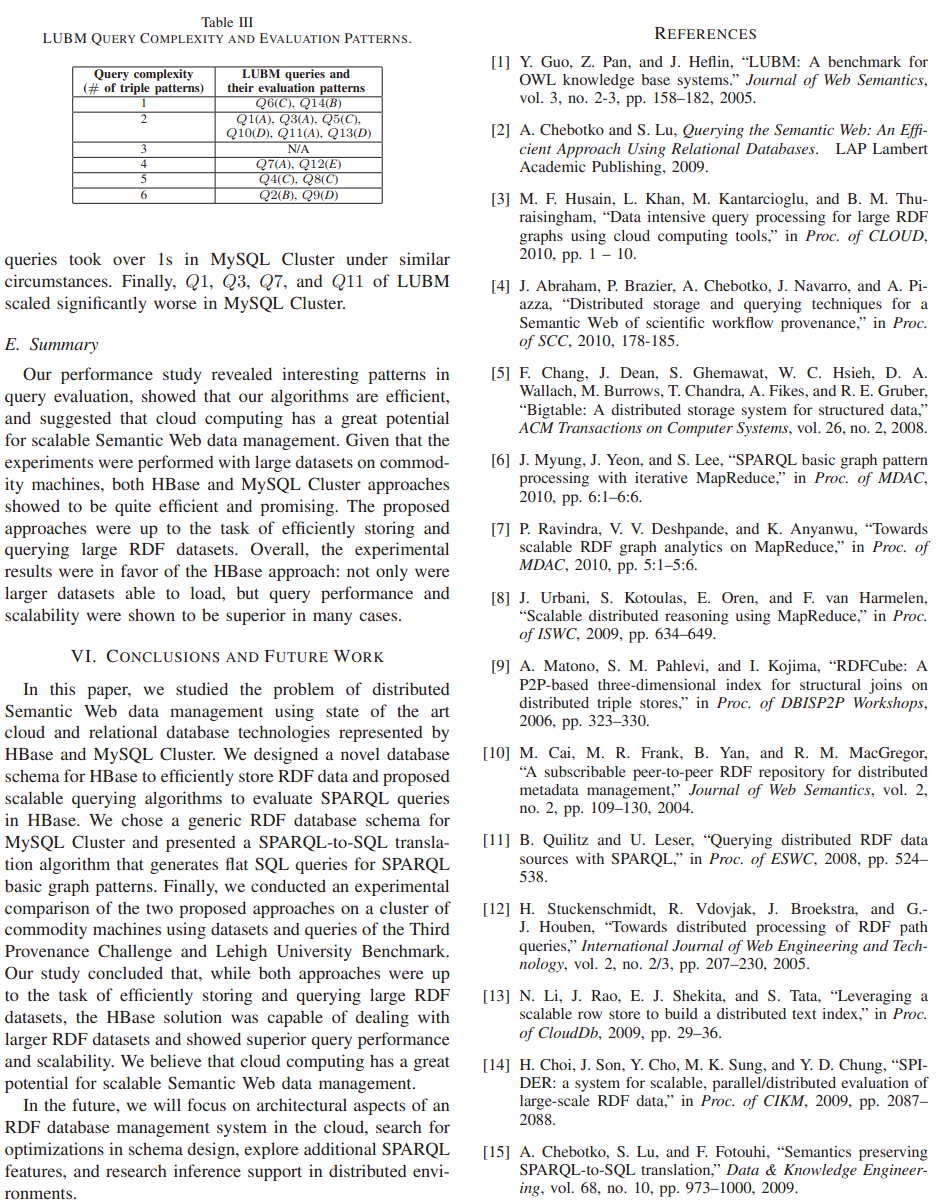
\includegraphics[scale=0.67]{photo/yingyu8.png}
\end{figure} 